\documentclass{book}
\renewcommand{\familydefault}{\sfdefault}

%\usepackage{libertine}
\usepackage{amsmath}
\usepackage{graphicx}	
\usepackage{amssymb}
\usepackage{epstopdf}
\usepackage{adjustbox}
\usepackage{array}
\usepackage{color}
\usepackage{pdflscape}
\usepackage{minted}
\usepackage{colortbl}
\usepackage{subcaption}

\usepackage{algorithm}
\usepackage{algorithmic}

\usepackage{tikz}

\usepackage[top=3cm,bottom=3cm,left=3cm,right=3cm,headsep=10pt,a4paper]{geometry} % Page margins

\usepackage{graphicx} 
\usepackage{titlepic}
%\usepackage{pstricks}

\usepackage[calcwidth]{titlesec}
\newlength\mylen
%\setlength\mylen{\dimexpr\oddsidemargin+1in+\hoffset\relax}
\setlength\mylen{\dimexpr\oddsidemargin+20pt+\hoffset\relax}
\titleformat{\section}
  {\normalfont\Large\bfseries}
  {\llap{\hspace*{-\mylen}\thesection\hfill}}{0em}{}
  [{\makebox[\linewidth][l]{%
    \hspace*{-\mylen}\rule{\dimexpr\textwidth+\mylen\relax}{1pt}}}]


\usepackage[framemethod=TikZ]{mdframed}
\mdfdefinestyle{MyFrame}{%
    linecolor=blue,
    outerlinewidth=2pt,
    roundcorner=20pt,
    innertopmargin=\baselineskip,
    innerbottommargin=\baselineskip,
    innerrightmargin=20pt,
    innerleftmargin=20pt,
    backgroundcolor=gray!50!white}

\mdfdefinestyle{cli}{%
    linecolor=none,
    outerlinewidth=2pt,
    roundcorner=5pt,
    innertopmargin=\baselineskip,
    innerbottommargin=\baselineskip,
    innerrightmargin=10pt,
    innerleftmargin=10pt,
    backgroundcolor=gray!10!white}


\mdfdefinestyle{aaa}{%
  topline=false,rightline=false,bottomline=false,
  frametitlerule=true,innertopmargin=10pt,
  outerlinewidth=3pt,outerlinecolor=gray,
  pstricksappsetting={\addtopsstyle{mdfouterlinestyle}{linestyle=dashed}},innerlinecolor=black,innerlinewidth=0pt}
 
%\usepackage{tikz}
%\usetikzlibrary{arrows,automata}

\usepackage{hyperref}
\hypersetup{
    colorlinks = true,
    linkcolor = {blue},
    linkbordercolor = {gray},
    citecolor = {blue}
}

\DeclareGraphicsRule{.tif}{png}{.png}{`convert #1 `dirname #1`/`basename #1 .tif`.png}

\newcommand{\CP}[2]{\text{{\bf P[}$ #1 \mid #2 ${\bf ]}}}
\newcommand{\PR}[1]{\text{{\bf P[}$#1${\bf]}}}
\newcommand{\F}{{\cal F}}
\newcommand{\M}{{\textsc{M}}}
\newcommand{\A}{{\textsc{A}}}



%\titlepic{\includegraphics[width=\textwidth]{joy-album.png}}
%\title{\huge Using \text{Joy}} 
%\author{David McGrew and others\\ \texttt{\{mcgrew\}@cisco.com} } 
%\institute{Cisco Systems, Inc. } 
%\date{\today}

%\definecolor{titlepagecolor}{cmyk}{1,.60,0,.40}
%\definecolor{titlepagecolor}{cmyk}{.16,.12,.13,.0}
\definecolor{titlepagecolor}{cmyk}{0,0,0,.3}
\definecolor{namecolor}{cmyk}{1,.50,0,.10} 
\definecolor{darkgray}{cmyk}{0,0,0,.27} 


\let\cleardoublepage=\clearpage

\begin{document}
%\pagecolor{titlepagecolor}
%\maketitle

\begin{titlepage}
\newgeometry{left=3cm} 
%\newgeometry{left=5cm} 
\pagecolor{titlepagecolor}
\noindent

\includegraphics[width=2.5in]{joy-icon.png}\\[-1em]
\color{white}
\rule{1\textwidth}{1pt} \\ \vspace{11pt}
\par
\noindent
\textbf{ \huge {\textsf{A Package for Capturing and Analyzing Network Data Features \newline\newline TLS Fingerprinting Addendum}}}
\vfill
\noindent
%{\huge \textsf{David McGrew, etc.}}
\vskip\baselineskip
\noindent
\textsf{ \huge \hfill Joy version 4.0}

\textsf{ \huge \hfill February 2019}
\end{titlepage}
\restoregeometry % restores the geometry
\pagecolor{white}

\frontmatter
\chapter{Preface}
\text{Joy} is a BSD-licensed open source software package for
collecting and analyzing network data, with a focus on network data
feature exploration.  This document shows how it can be used,
installed, built, and modified.  We hope that you find it useful, and
that you enjoy using it.  Please do understand that it is open source
software, with the following licensing terms:

\begin{quote}
Copyright \copyright \, 2019 Cisco Systems \\
All rights reserved. \\
 
Redistribution and use in source and binary forms, with or without
modification, are permitted provided that the following conditions are
met:
\begin{enumerate}
  \item Redistributions of source code must retain the above copyright
    notice, this list of conditions and the following disclaimer.
 
  \item Redistributions in binary form must reproduce the above
   copyright notice, this list of conditions and the following
   disclaimer in the documentation and/or other materials provided
   with the distribution.
 
   \item Neither the name of the Cisco Systems, Inc. nor the names of its
   contributors may be used to endorse or promote products derived
   from this software without specific prior written permission.
\end{enumerate}
   
 THIS SOFTWARE IS PROVIDED BY THE COPYRIGHT HOLDERS AND CONTRIBUTORS
 "AS IS" AND ANY EXPRESS OR IMPLIED WARRANTIES, INCLUDING, BUT NOT
 LIMITED TO, THE IMPLIED WARRANTIES OF MERCHANTABILITY AND FITNESS
 FOR A PARTICULAR PURPOSE ARE DISCLAIMED. IN NO EVENT SHALL THE
 COPYRIGHT HOLDERS OR CONTRIBUTORS BE LIABLE FOR ANY DIRECT,
 INDIRECT, INCIDENTAL, SPECIAL, EXEMPLARY, OR CONSEQUENTIAL DAMAGES
 (INCLUDING, BUT NOT LIMITED TO, PROCUREMENT OF SUBSTITUTE GOODS OR
 SERVICES; LOSS OF USE, DATA, OR PROFITS; OR BUSINESS INTERRUPTION)
 HOWEVER CAUSED AND ON ANY THEORY OF LIABILITY, WHETHER IN CONTRACT,
 STRICT LIABILITY, OR TORT (INCLUDING NEGLIGENCE OR OTHERWISE)
 ARISING IN ANY WAY OUT OF THE USE OF THIS SOFTWARE, EVEN IF ADVISED
 OF THE POSSIBILITY OF SUCH DAMAGE.

\end{quote}

%We gratefully acknowledge the support of our employer for the
%development of this package, and to the people who contributed to it,
%including Ellie Daw and Luke Valenta.
%
%\begin{quote}
%\textit{ -- the Joy team: Philip Perricone, Bill Hudson, Blake Anderson, Brian Long, and David McGrew}
%\end{quote}




\mainmatter

\tableofcontents


\chapter{Introduction}


\section{Overview}

TLS Fingerprinting is a technique that associates parameters extracted from a TLS ClientHello with a database of known fingerprints to provide visibility into the application and/or TLS library that created the session. Applications of TLS fingerprinting include malware detection \cite{anderson17deciphering}, minor-version operating system identification \cite{anderson17os}, and application identification. TLS fingerprinting has been studied since at least 2012 \cite{p0f2012tls}, and several open source databases have been released \cite{ja3,brotherston2015tls,kotzias2018tlsfingerprinting}. 

We extend the previous work on two fronts. First, as explained below, we developed a continuous pipeline that correlates endpoint and network data to ensure that our fingerprint database stays up-to-date. Second, we have focused on extracting all of the discriminating features in the ClientHello and providing more context when a TLS fingerprint matches a entry in our database. We use the automatic endpoint/network data correlation to provide lists of processes, along with their sha256 and prevalence, that we have seen associated with a TLS fingerprint. Additional details are provided in the schema definition (Chapter \ref{chapter:schema}).

Our open source contributions include a fingerprint database that is updated weekly, a Joy feature to generate fingerprint strings for TLS flows, and a set of python programs to identify TLS fingerprints in a packet capture or off a live network interface, generate new TLS fingerprints that can be contributed to the open source community, and a web-based user interface to visualize the results of TLS fingerprinting.

\section{TLS Fingerprinting}

Given a typical TLS session as shown in Figure \ref{fig:tls_session}, TLS fingerprinting extracts features from the first application data packet sent by the client, i.e., the \texttt{ClientHello}. The \texttt{ClientHello} message provides the server with a list of cipher suites and extensions that the client supports. The cipher suite list is ordered by preference of the client, and each cipher suite defines a set of cryptographic algorithms needed for TLS to operate. The TLS-defined cryptographic algorithms have real-world trade-offs, and this is reflected in different applications choosing to omit, include, or prefer cipher suites more aligned with their goals. The set of extensions provides additional information to the server that facilitates extended functionality, e.g., the Application Layer Protocol Negotiation extension indicates the list of application layer protocols that the client supports, e.g., \texttt{h2} and \texttt{http/1.1}. Some data carried in the extensions are useful for identifying the client application, while other extension data is session specific, e.g., the \texttt{SessionTicket} data. The string representation and unique identifier for our TLS fingerprints are in the following format:

\vspace{2mm}
\hspace{2mm}\texttt{(version)(cipher suites)((extensions)...)}
\vspace{2mm}

where:

\begin{itemize}
\item \texttt{(version)} is the hex representation of the advertised version, e.g., \texttt{(0303)} for TLS 1.2.
\item \texttt{(cipher suites)} is a hex list of the cipher suite offer vector, e.g., \texttt{(c02cc02bc030...0013)}.
\item \texttt{((extensions)...)} is a nested list of the hex-encoded extensions, where some extensions will have their data removed. Each individual extension with data looks like \texttt{(000b00020100)} where the first two bytes, \texttt{000b}, represent the extension hex code; the second two bytes, \texttt{0002}, represent the hex-encoded length of the data; and the last set of bytes, \texttt{0100}, represent the hex-encoded extension data. For extensions where we discard the data, we just report the hex-encoded extension type code, e.g., \texttt{(0000)}.
\end{itemize}

We include static extension data for \texttt{supported\_groups}, \texttt{ec\_point\_formats}, \texttt{status\_request}, \texttt{signature\_algorithms}, \texttt{application\_layer\_protocol\_negotiation}, \texttt{supported\_versions}, and \texttt{psk\_key\_exchange\_modes}.

\texttt{GREASE} \cite{grease} is a method to ensure TLS servers are properly handling unknown TLS cipher suites, extensions, and extension data. It is defined as a set of 16 hex codes, \texttt{\{0a0a,...,fafa\}}, that can be advertised in the ClientHello, but should never be chosen by the server. For our fingerprinting database, we normalize \texttt{GREASE} data to \texttt{0a0a}, but do not change the position of the data. Therefore, we avoid creating duplicate fingerprints based on the random \texttt{GREASE} hex code selection, but can still leverage the information about how the client is using \texttt{GREASE}. 

In our current studies, TLS 1.3 has improved the efficacy of TLS fingerprinting due to the added data features in the ClientHello. While, there are currently only 5 cipher suites defined for TLS 1.3, most TLS clients released in the foreseeable future will be backwards compatible with TLS 1.2, and will therefore offer many ``legacy" cipher suites. In addition to the 5 cipher suites, there are several new extensions. \texttt{supported\_versions} is an interesting TLS 1.3 extensions that allows us to differentiate between clients that supported earlier draft implementations of TLS 1.3.

\begin{figure}[t!]
        \centering
\resizebox{85mm}{!}{%                                                                                                                                     
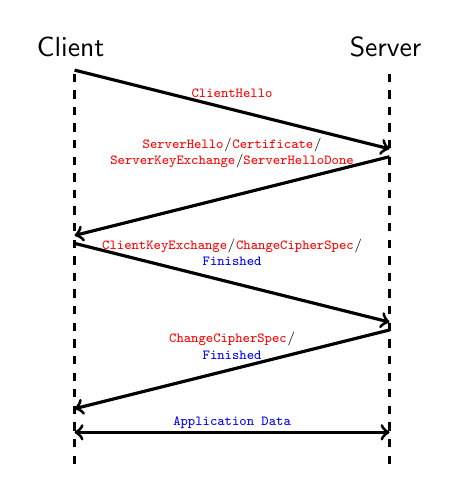
\begin{tikzpicture}
\node at (3.95,7.3) {\normalsize Server};
\node at (-0.05,7.3) {\normalsize Client};
\draw[line width=.4mm,dashed] (0,2) -- (0,7);
\draw[line width=.4mm,dashed] (4,2) -- (4,7);
\node at (2,6.7) {\tiny \textcolor{red}{\texttt{ClientHello}}};
\draw[line width=.4mm,->] (0,7) -- (4,6);
\node at (2,6.05) {\tiny \textcolor{red}{\texttt{ServerHello}}\hspace{.1mm}/\hspace{.1mm}\textcolor{red}{\texttt{Certificate}}\hspace{.1mm}/};
\node at (2,5.85) {\tiny \textcolor{red}{\texttt{ServerKeyExchange}}\hspace{.1mm}/\textcolor{red}{\texttt{ServerHelloDone}}};
\draw[line width=.4mm,->] (4,5.9) -- (0,4.9);
\node [align=center] at (2,4.77) {\tiny \textcolor{red}{\texttt{ClientKeyExchange}}\hspace{.1mm}/\hspace{.1mm}\textcolor{red}{\texttt{ChangeCipherSpec}}\hspace{.1mm}/};
\node [align=center] at (2,4.57) {\tiny \textcolor{blue}{\texttt{Finished}}};
\draw[line width=.4mm,->] (0,4.8) -- (4,3.8);
\node [align=center] at (2,3.58) {\tiny \textcolor{red}{\texttt{ChangeCipherSpec}}\hspace{.1mm}/};
\node [align=center] at (2,3.38) {\tiny \textcolor{blue}{\texttt{Finished}}};
\draw[line width=.4mm,->] (4,3.7) -- (0,2.7);
\node [align=center] at (2,2.52) {\tiny \textcolor{blue}{\texttt{Application Data}}};
\draw[line width=.4mm,<->] (0,2.4) -- (4,2.4);
\end{tikzpicture}
}
\caption{Graphical representation of a simplified TLS handshake and application data protocols. TLS fingerprinting uses features taken from the unencrypted \texttt{ClientHello} message.}
\label{fig:tls_session}
\end{figure}


\section{Data Collection}

The visibility gained by TLS fingerprinting is highly dependent on the underlying fingerprint database, and until now, generating this database was a manual process that was slow to update and was not reflective of real-world TLS usage. Building on work we first publically released in July 2016 \cite{anderson17deciphering}, we created a continuous process that fuses network telemetry with endpoint telemetry to build fingerprint databases automatically. This allows us to provide detailed information for a given fingerprint that is representative of how that fingerprint is used in the real-world, e.g., sha256's and lists of processes associated with a fingerprint sorted by the prevalence those applications were observed on the network's we monitor.


\chapter{Fingerprint Database Schema}
\label{chapter:schema}

\section{Overview}

The Fingerprint Schema is composed of 4 main sections. The first set of metadata fields provides some general information about the fingerprint, including unique keys that can be used to index the fingerprint entry in a dictionary. ``tls\_features" contains a human-readable description of the cipher suites, extensions, and extension data that was used to generate the TLS fingerprint. Finally, ``process/os\_info" contain information regarding the three most prevalent processes and operating systems we have observed using a given fingerprint.

\begin{figure}[H]\small
  \caption{Schema Overview}
  \label{figure:schema-overview}.
\begin{minted}{javascript}
{
  "str_repr": "...",                // Fingerprint metadata objects
  "md5_repr": "...",
  "source": ["..."],
  "max_implementation_date": "...", 
  "min_implementation_date": "...",
  "tls_features": {...},            // Human-readable description of TLS features
  "process_info": [...],            // List of associated process information objects
  "os_info": [...]                  // List of associated OS information objects
}
\end{minted}
\end{figure}


\section{Metadata}

The metadata fields are meant to provide a high-level summary of the fingerprint. ``str\_repr" is a string representation of the hex-values for the TLS features. It is reversible in the sense that there is a one-to-one correspondence with this representation and what you would observe on the wire, with a single caveat: all GREASE values are encoded as \texttt{0a0a}. ``md5\_repr" is the MD5 hash of the string representation, and source provides information about where a fingerprint was collected. We generate ``max/min\_implementation\_date" by first correlating every TLS parameter with the date of the RFC that first defined that parameter. From this list of dates, we report both the oldest and newest.

\begin{figure}[H]\small
  \caption{Metadata Fields}
  \label{figure:schema-metadata}.
\begin{minted}{javascript}
{
  "str_repr": "(0301)(00390038003300320035002f00ff)((0000)(0023))",
  "md5_repr": "89f96e9f19fd8754d9965ede7937a7b3",
  "source": ["Cisco"],
  "max_implementation_date": "2010-02",
  "min_implementation_date": "2002-06",
  ...
}
\end{minted}
\end{figure}

\section{TLS Features}

``tls\_features" is simply a human-readable description of the TLS features we use to construct the TLS fingerprint. The names should correspond to the names defined in the appropriate RFCs, but in some instances the parameters are unrecognized by a standards body and/or unknown to us. In these cases, we report an unknown identifier with the hex value.

\begin{figure}[H]\small
  \caption{TLS Fields}
  \label{figure:schema-tls}.
\begin{minted}{javascript}
{
  ...
  "tls_features": {
    "version": "TLS 1.0",
    "cipher_suites": [
      "TLS_DHE_RSA_WITH_AES_256_CBC_SHA",
      "TLS_DHE_DSS_WITH_AES_256_CBC_SHA",
      "TLS_DHE_RSA_WITH_AES_128_CBC_SHA",
      "TLS_DHE_DSS_WITH_AES_128_CBC_SHA",
      "TLS_RSA_WITH_AES_256_CBC_SHA",
      "TLS_RSA_WITH_AES_128_CBC_SHA",
      "TLS_EMPTY_RENEGOTIATION_INFO_SCSV"
    ],
    "extensions": [
      {"server_name": ""},
      {"session_ticket": ""}
    ]
  },
  ...
}
\end{minted}
\end{figure}

\section{Process Information}

We report the three most prevalent processes that we have seen using a given TLS fingerprint. For each process, we provide the name, sha256, and the prevalence. In Figure \ref{figure:schema-process}, a prevalence of 0.66 means that two thirds of the time, this specific fingerprint is observed coming from the process with the given sha256. Optionally, we have assigned a number of processes to application categories, which we report if available.

\begin{figure}[H]\small
  \caption{Process Information Fields}
  \label{figure:schema-process}.
\begin{minted}{javascript}
{
  ...
  "process_info": [
    {
      "process": "Python",
      "application_category": "programming",
      "prevalence": 0.66,
      "sha256": "A45244F6DCF841A6C165438BB16D074487A3BB1E83D705CBFB24690C3E09DCAE"
    },
    ...
  ],
  ...
}
\end{minted}
\end{figure}

\section{Operating System Information}

Similar to the process information object, we report the three most prevalent operating systems that we have seen using a given TLS fingerprint. We report the general operating system, the OS version and edition, and the prevalence we have seen the OS being used to generate the given TLS fingerprint.

\begin{figure}[H]\small
  \caption{OS Information Fields}
  \label{figure:schema-os}.
\begin{minted}{javascript}
{
  ...
  "os_info": [
    {
      "os": "Mac OS X",
      "os_version": "10.11.6",
      "os_edition": "El Capitan",
      "prevalence": 0.99
    },
    ...
  ]
}
\end{minted}
\end{figure}


\chapter{The \texttt{fingerprinter} Tool}

\texttt{fingerprinter.py} is a stand-alone python program that will read either a pcap file or a live network interface and assign a TLS fingerprint to every ClientHello it observes. If the TLS fingerprint has an exact match in the supplied database, then the process and OS information of the exact match will be reported. If the fingerprint is not in the database, but has a ``close" approximate match, the process and OS information of the approximate match will be reported. The approximate match will then be added to the in-memory version of the database to facilitate more efficient future lookups.


\section{Dependencies}

\begin{mdframed}[style=cli]
\begin{minted}{puppet}
pypcap >= 1.1.6
dpkt   >= 1.9.1
numpy  >= 1.14.2
\end{minted}
\end{mdframed}

\begin{mdframed}[style=cli]
\begin{minted}{bash}
pip install pypcap
pip install dpkt
pip install numpy
\end{minted}
\end{mdframed}

\section{Examples}

\begin{mdframed}[style=cli]
\begin{minted}{bash}
./fingerprinter.py test.pcap 
\end{minted}
\begin{minted}{javascript}
{"source_addr": "10.0.2.15", "dest_addr": "216.58.217.165", "source_port":
34496, "dest_port": 443, "timestamp": "2018-06-04 14:52:18.430744",
"fingerprint": {...}}
...
\end{minted}
\end{mdframed}

\section{Command Line Options}

\subsection{-i INPUT, --input=INPUT}
\begin{mdframed}[style=aaa]
Syntax:
  \begin{minted}{bash}
-i INPUT, --input=INPUT
  \end{minted}
\end{mdframed}
The command \texttt{-i INPUT} specifies the pcap file or interface.

\subsection{-f FP\_DB, --fp\_db=FP\_DB}
\begin{mdframed}[style=aaa]
Syntax:
  \begin{minted}{bash}
-f FP_DB, --fp_db=FP_DB
  \end{minted}
\end{mdframed}
The command \texttt{-f FP\_DB} specifies the location of fingerprint database (e.g., resources/fingerprint\_db.json.gz).

\subsection{-p PORT, --port=PORT}
\begin{mdframed}[style=aaa]
Syntax:
  \begin{minted}{bash}
-p PORT, --port=PORT
  \end{minted}
\end{mdframed}
The command \texttt{-p PORT} causes \texttt{fingerprinter} to only process traffic destined to port \texttt{PORT}.

\subsection{-o OUTPUT, --output=OUTPUT}
\begin{mdframed}[style=aaa]
Syntax:
  \begin{minted}{bash}
-o OUTPUT, --output=OUTPUT
  \end{minted}
\end{mdframed}
The command \texttt{-o OUTPUT} specifies the output file (the default is stdout).

\subsection{-l LOOKUP, --lookup=LOOKUP}
\begin{mdframed}[style=aaa]
Syntax:
  \begin{minted}{bash}
-l LOOKUP, --lookup=LOOKUP
  \end{minted}
\end{mdframed}
The command \texttt{-l LOOKUP} reports the database entry for a given fingerprint string, \texttt{str\_repr}.



\chapter{The \texttt{gen\_tls\_fingerprint} Tool}

\texttt{gen\_tls\_fingerprint.py} is a tool to facilitate the small-scale generation of TLS fingerprint databases that could be easily merged with the current open source fingerprint database hosted on the Joy github site. This program uses the output of the Joy network monitoring tool with two enabled features: \texttt{fpx} and \texttt{exe}. \texttt{fpx} reports the fingerprint string representation for each observed TLS flow containing a ClientHello, and \texttt{exe} hooks into the host operating system to report information about the process that generated the TLS flow. The resulting database can optionally include contributor information that would be integrated into the main open source fingerprint database.


\section{Dependencies}

\begin{mdframed}[style=cli]
\begin{minted}{puppet}
numpy >= 1.14.2
\end{minted}
\end{mdframed}

\begin{mdframed}[style=cli]
\begin{minted}{bash}
pip install numpy
\end{minted}
\end{mdframed}


\section{Examples}

\begin{mdframed}[style=cli]
\begin{minted}{bash}
./gen_tls_fingerprint.py fp_test.json.gz
\end{minted}
\begin{minted}{javascript}
{"str_repr": "...", "tls_features": {...}, "process_info": [...]}
{"str_repr": "...", "tls_features": {...}, "process_info": [...]}
{"str_repr": "...", "tls_features": {...}, "process_info": [...]}
...
\end{minted}
\end{mdframed}

\section{Command Line Options}

\subsection{-i INPUT, --input=INPUT}
\begin{mdframed}[style=aaa]
Syntax:
  \begin{minted}{bash}
-i INPUT, --input=INPUT
  \end{minted}
\end{mdframed}
The command \texttt{-i INPUT} specifies the Joy JSON output, with fpx=1 and exe=1.

\subsection{-o OUTPUT, --output=OUTPUT}
\begin{mdframed}[style=aaa]
Syntax:
  \begin{minted}{bash}
-o OUTPUT, --output=OUTPUT
  \end{minted}
\end{mdframed}
The command \texttt{-o OUTPUT} specifies the output file for the generated fingerprint database.

\subsection{-c CONTRIB\textunderscore INFO, --contrib\textunderscore info=CONTRIB\textunderscore INFO}
\begin{mdframed}[style=aaa]
Syntax:
  \begin{minted}{bash}
-c CONTRIB_INFO, --contrib_info=CONTRIB_INFO
  \end{minted}
\end{mdframed}
The command \texttt{-c CONTRIB\_INFO} specifies brief contributor information to be included in the fingerprint source.



\chapter{The \texttt{fingerprint\_ui} Tool}

\texttt{fingerprint\_ui.py} provides a simple, bottle-based user interface to inspect packet capture files. It will read the uploaded pcap file, extract the TLS fingerprint for all relevant connections, identify matches in the fingerprint database, and present the information in tabular form. A modal provides detailed information about the matching fingerprint and TLS parameters.

\section{Dependencies}

\begin{mdframed}[style=cli]
\begin{minted}{puppet}
bottle >= 0.12.13
pypcap >= 1.1.6
dpkt   >= 1.9.1
numpy  >= 1.14.2
\end{minted}
\end{mdframed}

\begin{mdframed}[style=cli]
\begin{minted}{bash}
pip install bottle
pip install pypcap
pip install dpkt
pip install numpy
\end{minted}
\end{mdframed}

\section{Examples}

\begin{mdframed}[style=cli]
\begin{minted}{bash}
./fingerprint_ui.py
\end{minted}
\end{mdframed}

\begin{figure}
	\centering % old scale=0.51 0.52, 0.44
   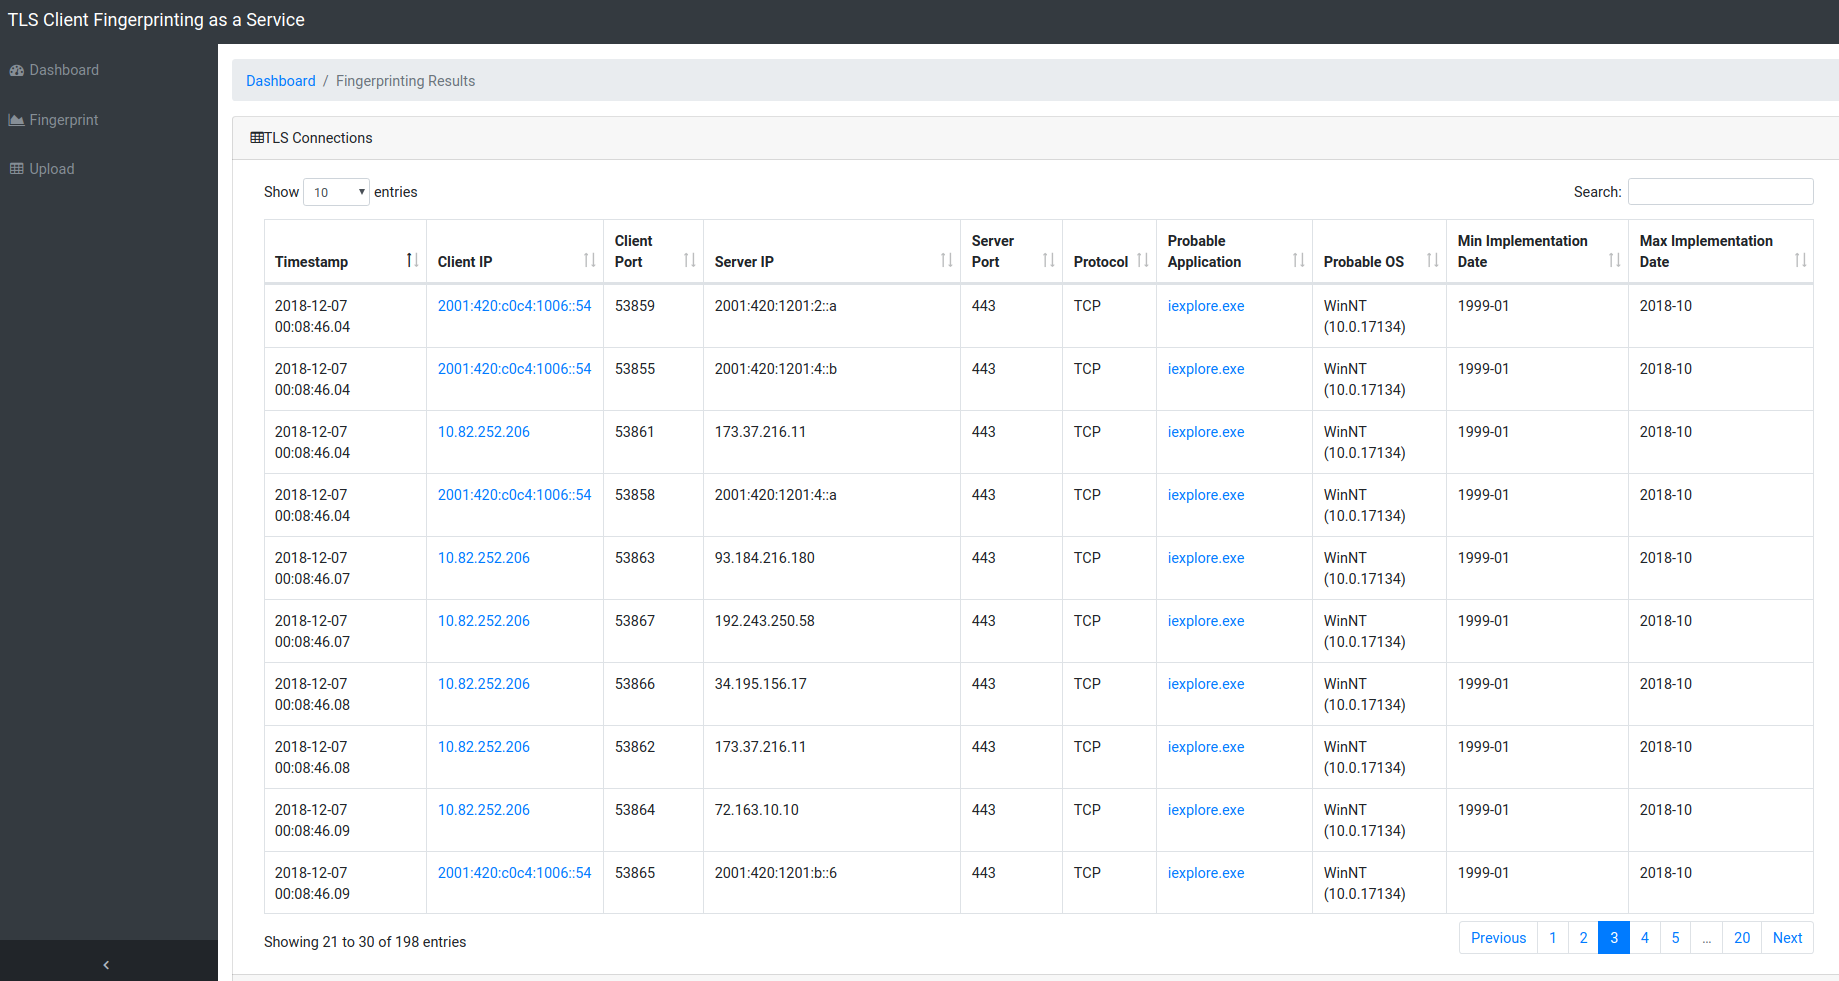
\includegraphics[scale=0.3]{ui_tls_fingerprinting_main.png}
	\caption{Fingerprint Results from Analyzing a pcap File.}
	\label{fig:ui-tls-fingerprint}
\end{figure}

\begin{figure}
	\centering % old scale=0.51 0.52, 0.44
   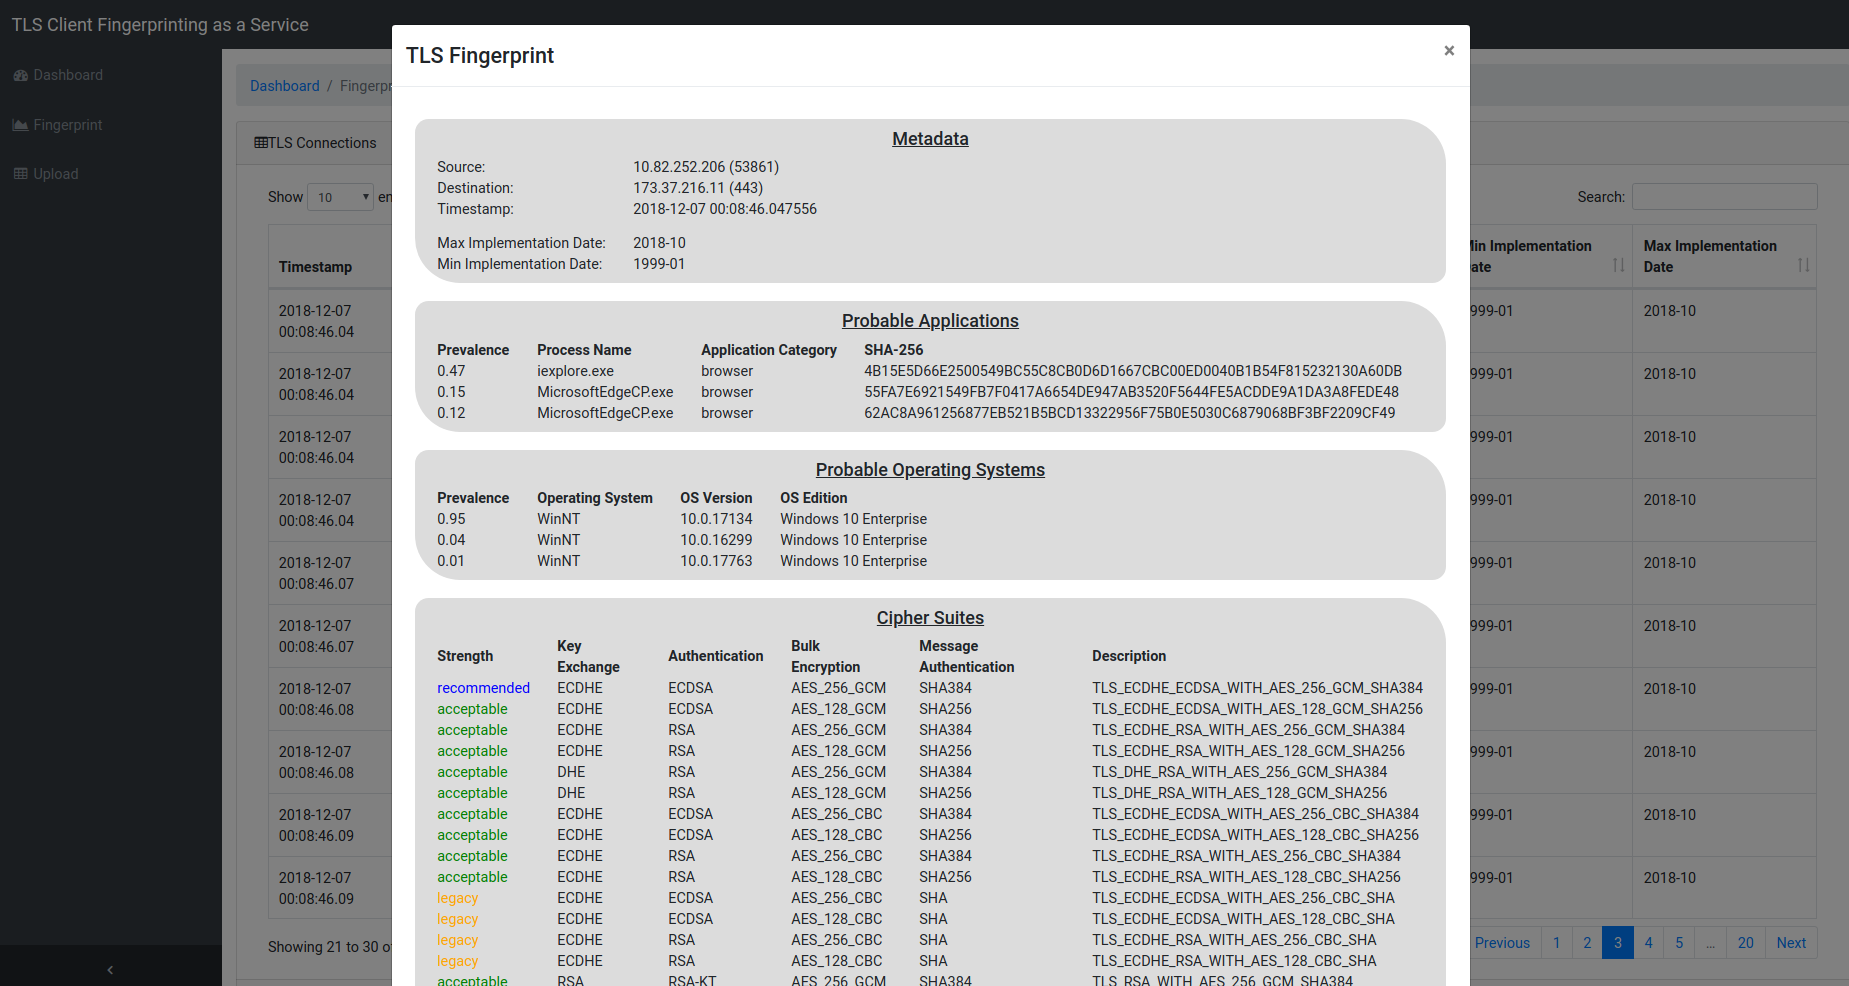
\includegraphics[scale=0.3]{ui_tls_fingerprinting.png}
	\caption{Fingerprint Inspection}
	\label{fig:ui-tls-fingerprint-inspection}
\end{figure}






\bibliography{joy}
\bibliographystyle{plain} 


\end{document}  
